\documentclass[11pt]{article}

\usepackage[T1]{fontenc}
\usepackage[english]{babel}
\usepackage{lmodern}
\usepackage{amsmath}
\usepackage{graphicx}
\usepackage{booktabs}
\usepackage{hyperref}
\usepackage{geometry}
\usepackage{float}
\usepackage[round]{natbib}
\usepackage{tipa}

\geometry{margin=1in}

\title{Forced Alignment Evaluation}
\author{
  Natural Language Processing Applications (5LN700) \\
  Uppsala University \\
  Student Name
}
\date{\today}

\begin{document}
\maketitle

\section{Introduction}
Forced alignment links a speech signal to a transcription by estimating when each linguistic unit starts and ends. This assignment aimed to compare two systems that provide word-level timing information: MAUS, a traditional HMM/GMM-based aligner, and Whisper, a neural end-to-end ASR system with word timestamps. Spoken language is harder to process than written language because of variation in pronunciation, reduction, noise, and timing \citep[p.~5]{jm3}. The practical goal of the assignment was therefore to examine how accurately the two systems place word boundaries and whether they show systematic timing bias.

Two kinds of data were used. First, one self-recorded English sentence was manually aligned in Praat and used for a small qualitative and quantitative comparison. Second, one Buckeye Corpus sample, \texttt{s1102a}, was used as a larger gold-standard dataset for quantitative evaluation.

\section{Data}
\subsection{Recording configurations}
The self-recorded material consisted of one English sentence with more than ten words: ``The development of women's football in Africa faces several challenges, including limited access to education, poverty amongst women, inequality and human rights abuses targeting women.'' The recording was stored as a \texttt{.wav} file and manually aligned in Praat at the word level. The manual gold alignment was saved as \texttt{manual\_alignment.TextGrid}. This gold file was then compared with one MAUS \texttt{.TextGrid} output and one Whisper \texttt{.json} output.

\subsection{Buckeye Corpus Subset}
The Buckeye part of the analysis used the file \texttt{s1102a}. The available Buckeye files included audio, orthographic transcription, word-level annotations, and phone-level annotations. In this report, only the word level was used, since the G part of the assignment focuses on word-level alignment. The gold-standard word boundaries were taken from the Buckeye \texttt{.words} file and then converted to CSV for comparison with MAUS and Whisper outputs. After matching and filtering, 628 word segments were retained for the quantitative analysis of \texttt{s1102a}.

\section{Methods}
\subsection{Forced Aligners}
The following systems were evaluated:
\begin{itemize}
    \item \textbf{MAUS}, a forced aligner based on more traditional acoustic modeling assumptions.
    \item \textbf{Whisper}, an end-to-end neural ASR system that also provides word-level timestamps.
\end{itemize}

\subsection{Data Extraction}
Separate Python scripts were written for MAUS \texttt{.TextGrid}, Whisper \texttt{.json}, and Buckeye \texttt{.words} files. All outputs were converted to a common CSV format with the columns \texttt{label}, \texttt{start}, and \texttt{end}. Time values were kept in seconds across all files. To make the systems comparable, labels were lowercased and non-lexical tags such as \texttt{<SIL>}, \texttt{<NOISE>}, \texttt{<VOCNOISE>}, and other annotation tags inside angle or curly brackets were removed. This step ensured comparable labels and comparable treatment of silence and noise.

\subsection{Evaluation Procedure}
Each gold word was matched to the output word with the same label that overlapped it most in time. If no appropriate match was found, that segment was excluded. Start-time and end-time signed errors were computed as predicted time minus gold time. Negative values therefore indicate that the system was early, whereas positive values indicate that it was late. Absolute errors were also computed by taking the absolute value of the signed error. The self-recorded sentence yielded 19 matched segments, and the Buckeye sample \texttt{s1102a} yielded 628 matched segments.

\section{Results}
\subsection{Overall Error Statistics}
Tables~\ref{tab:sentence_stats} and~\ref{tab:buckeye_stats} summarize mean, median, and spread for signed and absolute errors. In the present scripts, spread was operationalized as the standard deviation.

\begin{table}[H]
\centering
\small
\begin{tabular}{llrrr}
\toprule
System & Measure & Mean & Median & Spread \\
\midrule
MAUS & start error & 0.050 & 0.028 & 0.100 \\
MAUS & end error & 0.026 & -0.007 & 0.116 \\
MAUS & start abs.\ error & 0.070 & 0.038 & 0.087 \\
MAUS & end abs.\ error & 0.072 & 0.026 & 0.093 \\
Whisper & start error & -0.068 & 0.003 & 0.368 \\
Whisper & end error & -0.052 & -0.040 & 0.116 \\
Whisper & start abs.\ error & 0.178 & 0.105 & 0.327 \\
Whisper & end abs.\ error & 0.088 & 0.060 & 0.090 \\
\bottomrule
\end{tabular}
\caption{Summary statistics for the self-recorded sentence.}
\label{tab:sentence_stats}
\end{table}

\begin{table}[H]
\centering
\small
\begin{tabular}{llrrr}
\toprule
System & Measure & Mean & Median & Spread \\
\midrule
MAUS & start error & 0.013 & 0.003 & 0.043 \\
MAUS & end error & -0.002 & -0.003 & 0.054 \\
MAUS & start abs.\ error & 0.026 & 0.014 & 0.037 \\
MAUS & end abs.\ error & 0.026 & 0.014 & 0.047 \\
Whisper & start error & 0.040 & 0.068 & 0.208 \\
Whisper & end error & 0.118 & 0.075 & 0.194 \\
Whisper & start abs.\ error & 0.128 & 0.093 & 0.169 \\
Whisper & end abs.\ error & 0.134 & 0.080 & 0.183 \\
\bottomrule
\end{tabular}
\caption{Summary statistics for Buckeye \texttt{s1102a}.}
\label{tab:buckeye_stats}
\end{table}

For both datasets, MAUS produced smaller absolute errors than Whisper. This difference was especially clear for start-time errors.

\subsection{Systematic Bias}
The signed errors suggest somewhat different bias patterns across the two datasets. For the self-recorded sentence, MAUS had slightly positive mean signed errors for both start and end times, which suggests a small late bias on average. Whisper had negative mean signed errors for the sentence, which suggests an early bias there. For \texttt{s1102a}, both systems had positive mean start-time errors, and Whisper also had a clearly positive mean end-time error. This suggests that Whisper was more often late on the Buckeye material, whereas MAUS stayed much closer to zero overall.

\subsection{Regression Analysis}
The regression model used start-time signed error as the dependent variable and gold-segment duration as the sole predictor, following the assignment instructions. The purpose was to test whether longer gold words tend to be associated with systematically earlier or later start boundaries.

For the self-recorded sentence, MAUS showed almost no linear relationship between duration and signed start error (slope $= 0.0003$, $R^2 \approx 0.0000$, slope \textit{p} $= 0.9980$). This means that word duration did not predict MAUS start-time bias in this very small sample. Whisper showed a larger positive slope ($0.7584$) and a higher $R^2$ ($0.2356$), and the slope \textit{p}-value was $0.0352$. In this case, the positive slope means that longer words tended to be associated with later predicted start times. However, the result is still based on only 19 matched words, so it should be interpreted cautiously.

\begin{figure}[H]
\centering
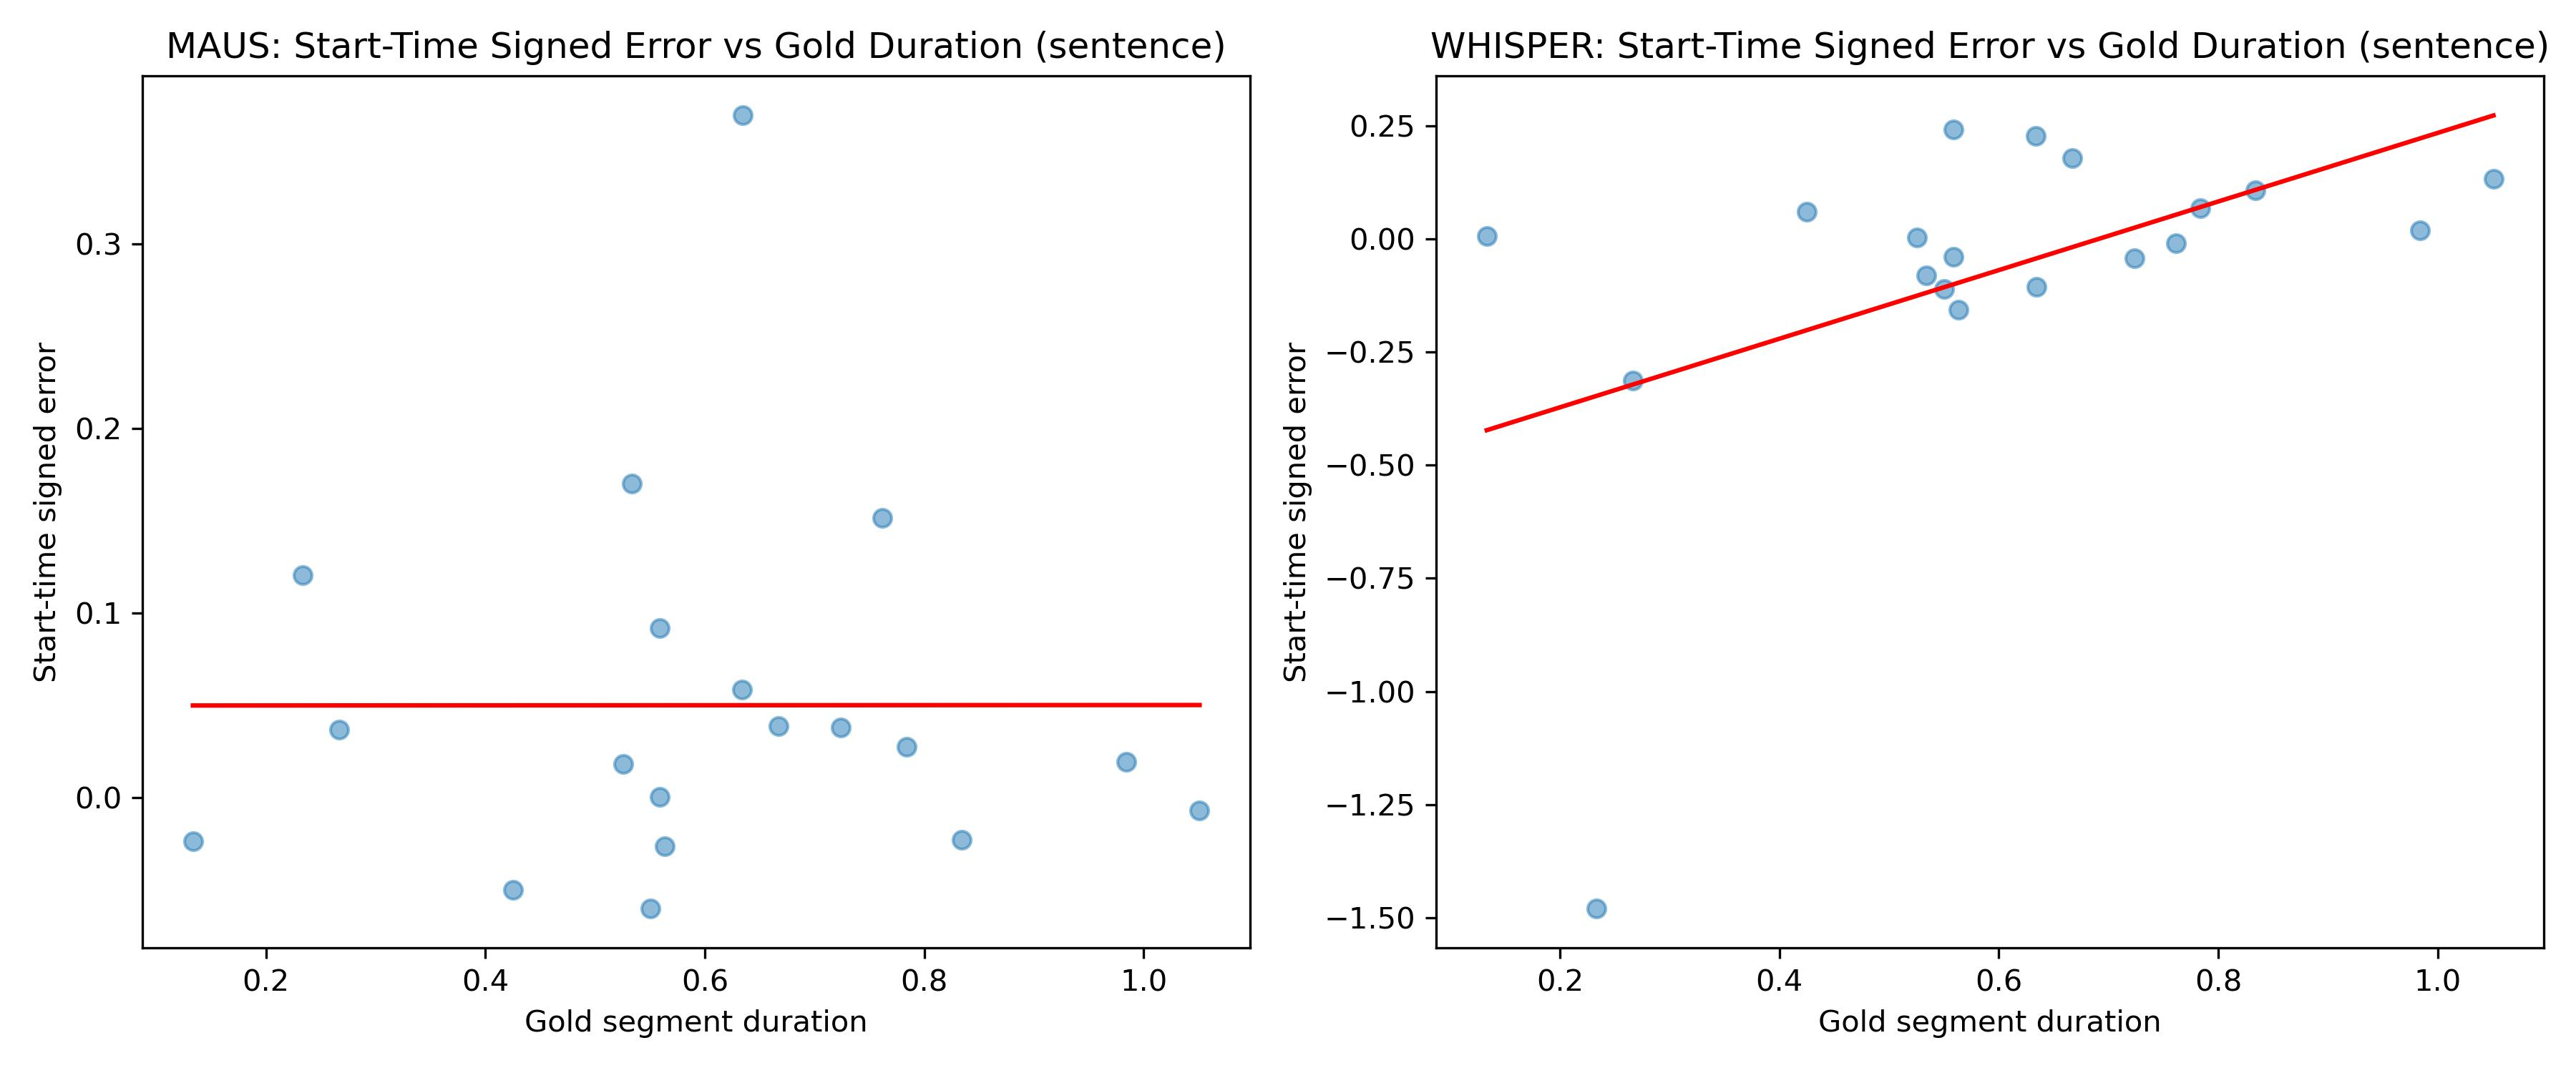
\includegraphics[width=\textwidth]{results/sentence_regression_plot.jpg}
\caption{Regression plots for the self-recorded sentence. The x-axis shows gold-segment duration and the y-axis shows start-time signed error. The red line is the fitted linear regression line.}
\label{fig:sentence_regression}
\end{figure}

For Buckeye \texttt{s1102a}, both systems again showed weak relationships in practical terms. MAUS had slope $= 0.0545$, slope \textit{p} $< 0.001$, and $R^2 = 0.0393$, while Whisper had slope $= 0.1274$, slope \textit{p} $= 0.0166$, and $R^2 = 0.0091$. The positive slopes indicate that longer words tended to be associated with later predicted start times for both systems. However, the very low $R^2$ values show that gold-segment duration explains only a very small proportion of the variance in start-time signed error. In other words, duration had a statistically detectable effect here, but it was not a strong predictor of alignment bias.

\begin{figure}[H]
\centering
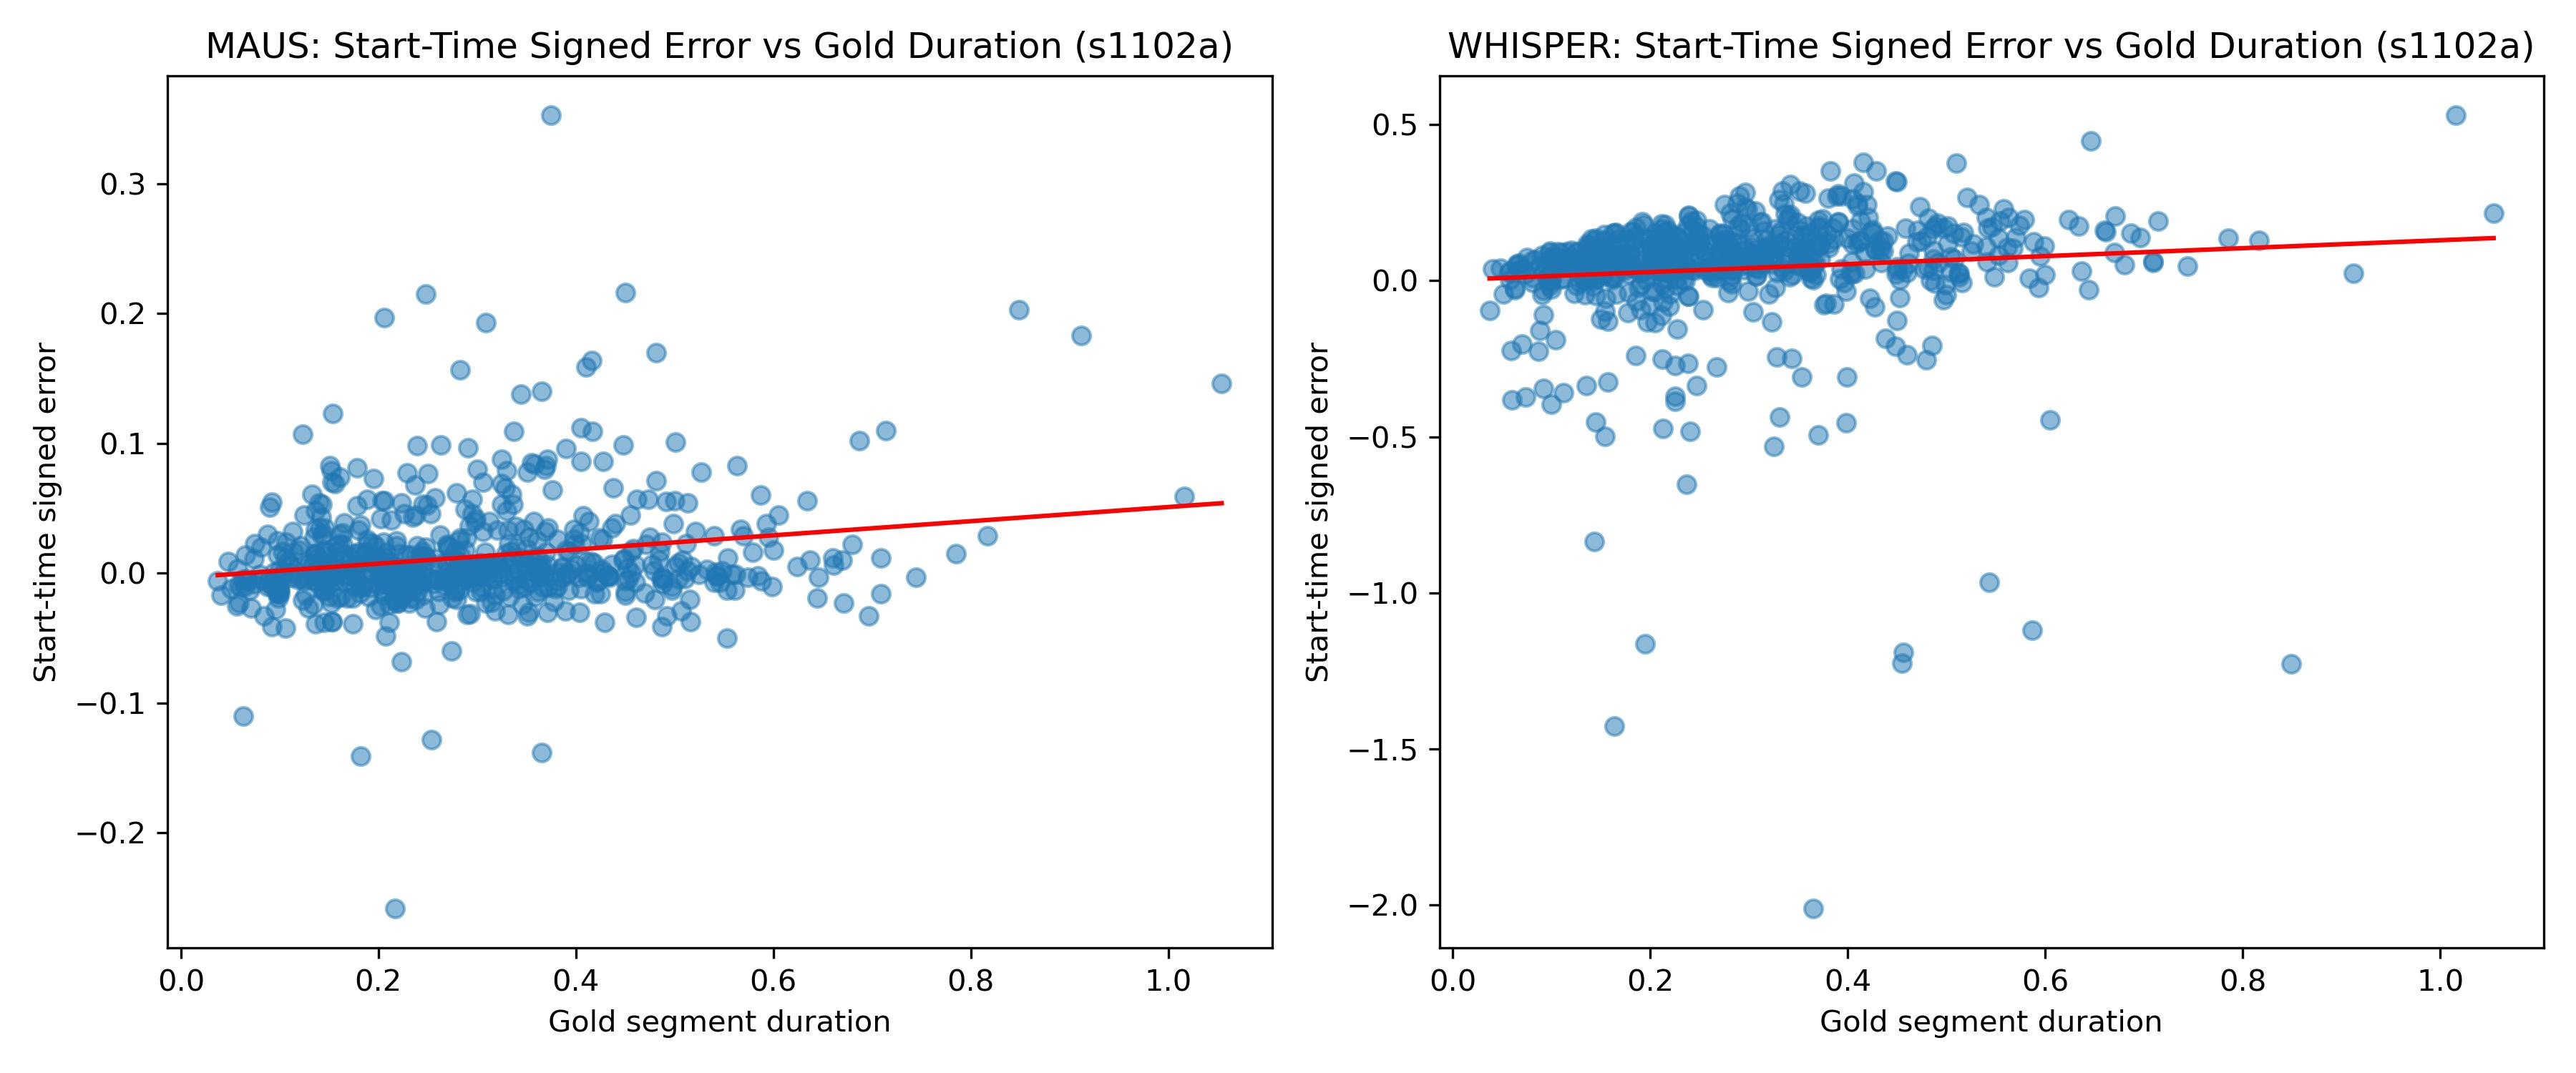
\includegraphics[width=\textwidth]{results/s1102a_regression_plot.jpg}
\caption{Regression plots for Buckeye \texttt{s1102a}. The x-axis shows gold-segment duration and the y-axis shows start-time signed error. The red line is the fitted linear regression line.}
\label{fig:s1102a_regression}
\end{figure}

Figures~\ref{fig:sentence_regression} and~\ref{fig:s1102a_regression} support the numerical regression results. In both datasets, the fitted lines are relatively shallow, especially for MAUS, which is consistent with the low $R^2$ values. In this model, the reported \textit{p}-values refer to the coefficient estimates, especially the slope coefficient, and test the null hypothesis that the coefficient is equal to zero. They do not measure the size of the effect itself. Therefore, the slope estimate shows the direction and size of the relationship, the \textit{p}-value shows the evidence against a zero slope, and $R^2$ shows how much variance in signed start-time error is explained by duration.

\section{Discussion}
Overall, MAUS was the more accurate system in this evaluation. On both the sentence-level gold data and the Buckeye sample, MAUS produced lower mean and median absolute errors than Whisper. This suggests that MAUS placed word boundaries more consistently and more precisely. Whisper, in contrast, often produced larger start-time errors and more unstable timing, especially on the self-recorded sentence.

One likely reason is that MAUS is designed specifically for forced alignment, whereas Whisper is primarily an ASR system and only secondarily provides timestamps. Whisper may therefore produce reasonable lexical output while still placing boundaries less accurately. Another reason is that Whisper occasionally split, merged, or misrecognized words, which increased the number of excluded segments and reduced comparability.

There are also important limitations. First, only one self-recorded sentence and one Buckeye sample were analyzed. Second, the Buckeye subset was restricted to \texttt{s1102a} in the final analysis. Third, the regression model used only one predictor, so it could capture only a small part of the timing variation. Finally, even where slope \textit{p}-values were statistically significant, the corresponding $R^2$ values remained very low, so statistical significance should not be confused with strong predictive power.

\section{Summary}
This assignment compared MAUS and Whisper on word-level alignment using both a manually aligned sentence and one Buckeye sample. The outputs were converted into a common format, matched to gold segments, and evaluated with signed and absolute timing errors. MAUS showed lower absolute errors and generally more stable alignment than Whisper. Signed errors further suggested that timing bias varied by system and dataset. The regression analyses showed that gold-segment duration alone explained little of the variation in signed start-time error. Overall, the assignment showed that different systems may provide word timestamps, but those timestamps can differ substantially in quality and bias.

\section*{VG Extension (if applicable)}
Not included in this report.

\bibliographystyle{plainnat}
\bibliography{references}

\end{document}
